\documentclass[11pt]{article}

\setlength{\textwidth}{6in}
\setlength{\oddsidemargin}{0.25in}
\setlength{\textheight}{9.0in}
\setlength{\topmargin}{-0.75in}

% common LaTeX macros
%
% Last modified: 03-02-2007
%

\usepackage{times}
%-------------------------
% the following magic makes the tt font in math mode be the same as the
% normal tt font (i.e., Courier)
%
\SetMathAlphabet{\mathtt}{normal}{OT1}{pcr}{n}{n}
\SetMathAlphabet{\mathtt}{bold}{OT1}{pcr}{bx}{n}
%-------------------------

\usepackage{amsmath}
\usepackage{amssymb} % for \pitchfork

\newcommand{\NOTE}[1]{%
  \par\leavevmode\noindent\textbf{[[ #1 ]]}\par\leavevmode\noindent}
\newcommand{\CUT}[1]{}
\newcommand{\SIDENOTE}[1]{%
  \marginpar{\tiny\raggedright{#1}}}

\newcommand{\appref}[1]{Appendix~\ref{#1}}
\newcommand{\chapref}[1]{Chapter~\ref{#1}}
\newcommand{\secref}[1]{Section~\ref{#1}}
\newcommand{\tblref}[1]{Table~\ref{#1}}
\newcommand{\figref}[1]{Figure~\ref{#1}}
\newcommand{\listingref}[1]{Listing~\ref{#1}}
\newcommand{\pref}[1]{{page~\pageref{#1}}}
\newcommand{\defref}[1]{Definition~\ref{#1}}
\newcommand{\ruleref}[1]{Rule~\ref{#1}}

\newcommand{\eg}{{\em e.g.}}
\newcommand{\cf}{{\em cf.}}
\newcommand{\ie}{{\em i.e.}}
\newcommand{\etc}{{\em etc.\/}}
\newcommand{\naive}{na\"{\i}ve}
\newcommand{\ala}{{\em \`{a} la\/}}
\newcommand{\etal}{{\em et al.\/}}
\newcommand{\role}{r\^{o}le}
\newcommand{\vs}{{\em vs.}}
\newcommand{\forte}{{fort\'{e}\/}}

%
% language names
\newcommand{\Cplusplus}{\mbox{C\hspace{-.05em}\raisebox{.4ex}{\tiny\bf ++}}}
\newcommand{\Cmm}{\mbox{C\hspace{-.05em}\raisebox{.4ex}{\small\textbf{{-}{-}}}}}
\newcommand{\csharp}{\textsc{C\#}}
\newcommand{\C}{\textsc{C}}
\newcommand{\Ckit}{\textsc{Ckit}}
\newcommand{\java}{\textsc{Java}}
\newcommand{\loom}{\textsc{Loom}}
\newcommand{\moby}{\textsc{Moby}}
\newcommand{\minimoby}{\textsc{MiniMoby}}
\newcommand{\micromoby}{\textsc{microMoby}}
\newcommand{\MOC}{\textsc{MOC}}
\newcommand{\ml}{\textsc{ML}}
\newcommand{\sml}{\textsc{SML}}
\newcommand{\smlnj}{\textsc{SML/NJ}}
\newcommand{\mlj}{\textsc{MLj}}
\newcommand{\cml}{\textsc{CML}}
\newcommand{\pml}{\textsc{PML}}
\newcommand{\ocaml}{\textsc{OCaml}}
\newcommand{\mlkk}{\textsc{ML2000}}
\newcommand{\haskell}{\textsc{Haskell}}
\newcommand{\mltwok}{\textsc{ML2000}}
\newcommand{\scala}{\textsc{Scala}}
\newcommand{\perl}{\textsc{Perl}}
\newcommand{\scheme}{\textsc{Scheme}}
\newcommand{\unix}{\textsc{Unix}}
\newcommand{\smalltalk}{\textsc{Smalltalk}}
\newcommand{\self}{\textsc{Self}}

%
% font commands
\providecommand{\bftt}[1]{{\ttfamily\bfseries{}#1}}
\providecommand{\ittt}[1]{{\ttfamily\itshape{}#1}}
\providecommand{\kw}[1]{\bftt{#1}}
\providecommand{\nt}[1]{{\rmfamily\itshape{#1}}}
\providecommand{\term}[1]{{\sffamily{#1}}}
%
% math-mode versions
\providecommand{\mkw}[1]{\ensuremath{\text{\kw{#1}}}}
\providecommand{\mnt}[1]{\ensuremath{\text{\nt{#1}}}}
\providecommand{\mterm}[1]{\ensuremath{\text{\term{#1}}}}

% braces (in math mode)
\newcommand{\LCB}{\mkw{\{}}
\newcommand{\RCB}{\mkw{\}}}

% underscore
\newcommand{\US}{\char`\_}

%%%%%
% Some common math notation
%

% double brackets
\newcommand{\LDB}{\ensuremath{[\mskip -3mu [}}
\newcommand{\RDB}{\ensuremath{]\mskip -3mu ]}}

\newcommand{\dom}{\ensuremath{\mathrm{dom}}}
\newcommand{\rng}{\ensuremath{\mathrm{rng}}}

% sets
\newcommand{\SET}[1]{\ensuremath{\{#1\}}}
\newcommand{\Fin}{\textrm{Fin}}     % finite power set
\newcommand{\DISJOINT}[2]{\ensuremath{#1 \pitchfork #2}}
\newcommand{\finsubset}{\mathrel{\stackrel{\textrm{fin}}{\subset}}}


% finite maps
\newcommand{\finmap}{\mathrel{\stackrel{\textrm{fin}}{\rightarrow}}}
\newcommand{\MAP}[2]{\SET{#1 \mapsto #2}}
\newcommand{\EXTEND}[2]{\ensuremath{#1{\pm}#2}}
\newcommand{\EXTENDone}[3]{\EXTEND{#1}{\MAP{#2}{#3}}}
\newcommand{\SUBST}[3]{\ensuremath{#1[#2\mapsto{}#3]}}
\newcommand{\SUBSTTWO}[5]{\ensuremath{#1[#2\mapsto{}#3,#4\mapsto{}#5]}}


% timestamp
\newcount\timeHH
\newcount\timeMM
\timeHH=\time
\divide\timeHH by 60
\timeMM=\time
\count255=\timeHH
\multiply\count255 by -60 \advance\timeMM by \count255
\newcommand{\timestamp}{%
  \today{} ---
  \ifnum\timeHH<10 0\fi\number\timeHH\,:\,\ifnum\timeMM<10 0\fi\number\timeMM}


\usepackage{graphicx}
\usepackage{listings}

\title{VProc protocol}
\author{The Manticore Group}
\date{Draft of \today}

\begin{document}
\maketitle

\section{Overview}
This document describes the protocol for managing vprocs.

\section{Signaling \& sleeping}\label{sec:signaling-and-sleeping}
This section presents two alternative signaling protocols for vprocs.
Both protocols have their advantages, and this section makes an attempt to understand
which is most appropriate for the Manticore implementation.
The rest of this section is structured as follows.
In this secion we outline the interface and semantics of the protocol.
Section \ref{sec:protocol1} describes the first protocol, and section
\ref{sec:protocol2} describes the second protocol.
Then \secref{sec:conclusion} compares the protocols.

\paragraph{Signals}
A signal is a fiber paired with fiber-local storage.
To handle a signal, a vproc initializes the fiber-local storage and runs the fiber to completion.

\paragraph{Landing pad}
The \emph{landing pad} is a lock-free linked list of incoming signals.
Each vproc owns a landing pad, and has access to all the other remote landing pads.
The landing pad supports two operations.
\begin{enumerate}
  \item Push a message on a remote landing pad.
  \item Pop all messages from the local landing pad.
\end{enumerate}

\paragraph{Sleeping}
When there is nothing to do, a vproc enters a temporary sleeping state, which lasts until a
signal arrives on the vproc's landing pad or a global garbage collection is initiated by some other
vproc.
We avoid busy waiting by waiting on a condition variable provided by the Pthreads
library.
Unfortunately, the fact that the landing pad is a lock-free data structure causes
a problem.
Signals may arrive after the vproc has checked the landing pad but before the vproc has
begun waiting on the condition variable.
Thus, there is a potential race condition that would allow the vproc to wait indefinitely,
even when work becomes available.
Our protocols must address this race condition by using some additional
synchronization.

\paragraph{Vproc operations}
Below are the two operations that the vproc protocol must provide.
The Sleep operation puts the host vproc to sleep;
the Send operation places the provided signal on vp's landing pad.
\lstset{language=C}
\lstset{commentstyle=\textit}
\begin{lstlisting}
void Sleep (VProc_t *host);
void Send (VProc_t *vp, Fiber_t *k, Value_t *fls);
\end{lstlisting}
We choose to minimize the synchronization overhead of Send even at the expense of
increasing the overhead of Sleep.
The rationale is that, in the common case, the Sleep operation affects idle vprocs, whereas
the Send function affects working vprocs.

\paragraph{Vproc components}
The per vproc structure VProc\_t contains four components that are relevant to this discussion.
However, the sleeping flag is only necessary for the first protocol.
\lstset{language=C}
\lstset{commentstyle=\textit}
\begin{lstlisting}
struct struct_vproc {
    ...
    Value_t     landingPad;       // landing pad
    Mutex_t	lock;  		  // lock for VProc state
    Cond_t	wait;		  // for waiting when idle
    Bool_t      sleeping;         // sleeping flag
    ...
};
typedef struct struct_vproc VProc_t;
\end{lstlisting}

\section{Protocol 1}\label{sec:protocol1}

\paragraph{Landing pad representation}
The landing pad is represented by one of the following values, where EMPTY
denotes an empty stack, k is a fiber, fls is fiber-local storage, and stk
is a queue item.
\lstset{language=C}
\lstset{commentstyle=\textit}
\begin{lstlisting}
EMPTY
QueueItem(k, fls, stk)
\end{lstlisting}

\paragraph{Send}
The Send operation (\figref{fig:protocol1-send}) has two phases: first it repeatedly attempts to place a
signal on the landing pad (lines 3-8), and once successful, it checks
whether the vproc needs to be woken up (lines 10-12).

\begin{figure}
\lstset{language=C}
\lstset{commentstyle=\textit}
\lstset{numbers=left}
\begin{lstlisting}
void Send (VProc_t *vp, Fiber_t *k, Value_t *fls)
{
  while (true) {
    Value_t *stk = vp->landingPad;
    Value_t *newStk = Promote(QueueItem(k, fls, stk));
    Value_t *x = CAS(&(vp->landingPad), stk, newStk);
    if (x != stk) {
      continue;
    } else {
      if (vp->sleeping) {
        CondSignal(&(vp->wait));
      }
      return;
    }
  }
}
\end{lstlisting}
\caption{Protocol 1 \texttt{Send} operation.}\label{fig:protocol1-send}
\end{figure}

\paragraph{Sleep}
The Sleep operation (\figref{fig:protocol1-sleep}) puts the vproc to sleep by 
setting the sleeping flag to true and subsequently waiting until the landing
pad becomes nonempty.
One subtelty is that the assignment to sleeping (line 4) must be visible
to other vprocs before checking the landing pad (line 5).
So on a processor without sequential consistency, we need an instruction that flushes 
the write buffer.
An atomic compare-and-swap at line 4 would suffice, but any lighter-weight instruction
that flushes the write buffer is preferable.

\paragraph{Correctness}
The correctness of this protocol becomes apparent with the following observation.
If the vproc sees that its landing pad is empty (line 6 of \figref{fig:protocol1-send}), 
then the vproc appears to be sleeping to the other vprocs.
Thus, it must be the case that all subsequent sends to that vproc are garanteed to
wake the vproc from its sleeping state (line 11 of \figref{fig:protocol1-send}).

\begin{figure}
\lstset{language=C}
\lstset{commentstyle=\textit}
\lstset{numbers=left}
\begin{lstlisting}
void Sleep (VProc_t *host)
{
  MutexLock(&(host->lock));
    host->sleeping = true;
    /* Flush all pending writes */
    while (host->landingPad == EMPTY)
      CondWait(&(host->wait), &(host->lock));
    host->sleeping = false;
  MutexUnlock(&(host->lock));
}
\end{lstlisting}
\caption{Protocol 1: \texttt{Sleep} operation.}\label{fig:protocol1-sleep}
\end{figure}

\section{Protocol 2}\label{sec:protocol2}

\paragraph{Landing pad representation}
The landing pad is represented the same way as in protocol 1, except that it 
contains an additional SLEEPING state.
\lstset{language=C}
\lstset{commentstyle=\textit}
\begin{lstlisting}
EMPTY
SLEEPING
QueueItem(k, fls, stk)
\end{lstlisting}

\paragraph{Send}
The Send (\figref{fig:protocol2-sleep}) operation consists of two paths: the path where the remote vproc
is awake (lines 6-11), and the path where the remote vproc is potentially
sleeping (lines 13-21).
In the former path, we repeatedly attempt to place a signal on the remote
vproc's landing pad.
In the latter path, we lock the remote vproc's state.
If the vproc is still sleeping, then we place the signal on its landing
pad and wake the vproc.

\begin{figure}
\lstset{language=C}
\lstset{commentstyle=\textit}
\lstset{numbers=left}
\begin{lstlisting}
void Send (VProc_t *vp, Fiber_t *k, Value_t *fls)
{
  while (true) {
    Value_t *stk = vp->landingPad;
    if (stk != SLEEPING) {
      Value_t *newStk = Promote(QueueItem(k, fls, stk));
      Value_t *x = CAS(&(vp->landingPad), stk, newStk);
      if (x == stk)
	return;
      else
	continue;
    } else {            /* (stk == SLEEPING) */
      MutexLock(&(vp->lock));
        if (vp->landingPad != SLEEPING) {
          MutexUnlock(&(vp->lock));
          continue;
        }
        vp->landingPad = Promote(QueueItem(k, fls, EMPTY));
        CondSignal(&(vp->wait));
      MutexUnlock(&(vp->lock));
      return;
    }
  }
}
\end{lstlisting}
\caption{Protocol 2 \texttt{Send} operation.}\label{fig:protocol2-send}
\end{figure}

\paragraph{Sleep}
The Sleep operation (\figref{fig:protocol2-sleep}) acquires the lock
and then attempts to mark the state as sleeping.
If this step succeeds, the vproc sleeps until a the landing pad becomes
nonempty.

\begin{figure}
\lstset{language=C}
\lstset{commentstyle=\textit}
\lstset{numbers=left}
\begin{lstlisting}
void Sleep (VProc_t *host)
{
  MutexLock(&(vp->lock));
    Value_t *x = CAS(&(vp->landingPad), EMPTY, SLEEPING);
    while (vp->landingPad == SLEEPING)
      CondWait(&(vp->wait), &(vp->lock));
  MutexUnlock(&(vp->lock));
}
\end{lstlisting}
\caption{Protocol 2: \texttt{Sleep} operation.}\label{fig:protocol2-sleep}
\end{figure}

\paragraph{Correctness}
The key observation of correctness is that if the vproc succeeds in entering a sleep
state (line 4 \figref{fig:protocol2-sleep}), then one and only one other vproc sees 
that this is the case (line 14 of \figref{fig:protocol2-send}).
Thus, this other vproc subsequently wakes the sleeping vproc when it sends a signal.

\section{Conclusion}\label{sec:conclusion}
Protocol 1 is conceptually simpler and requires fewer lines of code.
Protocol 2, however, is likely to be faster on the common case, where the vproc is
already awake.
In this case, protocol 2 makes one less remote memory reference than protocol 1.

\CUT{
\begin{figure}[tp]
  \begin{center}
    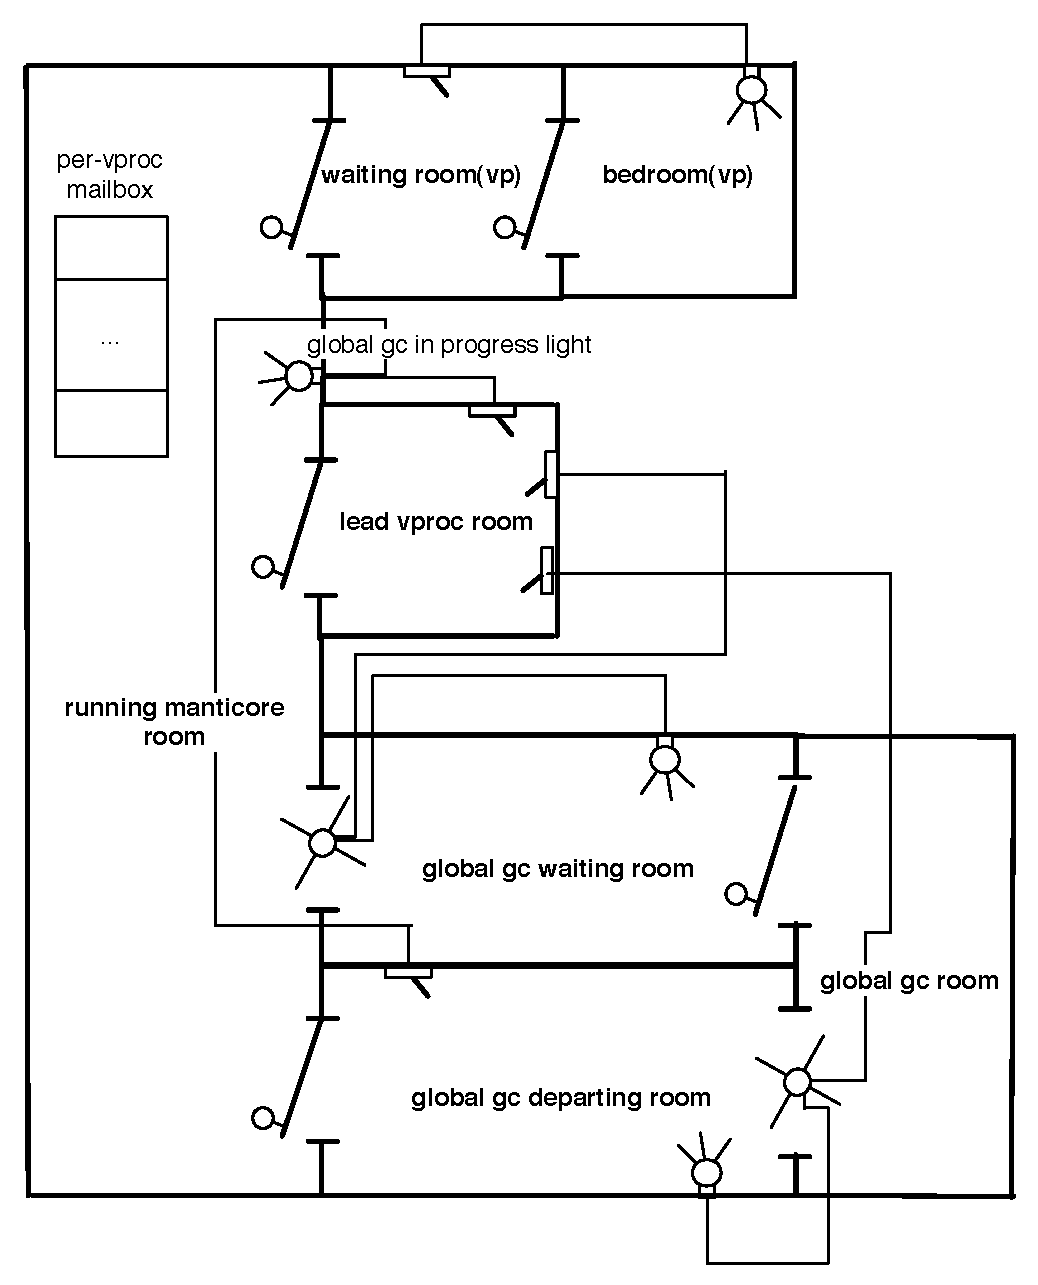
\includegraphics[scale=0.7]{pictures/vproc-protocol}
  \end{center}%
  \caption{Layout of the VProc protocol.}
  \label{fig:vproc-protocol}
\end{figure}%

\section{Messaging}

\paragraph{\texttt{Send(vp, msg)}}

\begin{description}
\item [\textit{Precondition:}] \textit{It is the case that} \texttt{vp} $\neq$ \texttt{host\_vproc} \textit{(a vproc cannot send a message to itself)}
\end{description}

\begin{enumerate}
  \item Walk to \texttt{vp}'s desk and open the mailbox.
    \begin{enumerate}
      \item If there is a \texttt{SLEEPING} message, place \texttt{msg} in the mailbox and go to step 2.
      \item Otherwise, place \texttt{msg} in the mailbox and exit the subroutine.
    \end{enumerate}
  \item Walk into \texttt{vp}'s \textbf{waiting room}.
    \begin{enumerate}
      \item If the waiting-room switch is off, then do the following. \textit{(\textbf{Invariant:}} \texttt{vp} \textit{is on its way to the waiting room.)}
        \begin{enumerate}
          \item Flip the waiting-room switch on.
          \item Return to the local desk.
          \item Exit the subroutine.
        \end{enumerate}
      \item If the waiting-room switch is on, then go to step 3. \textit{(\textbf{Invariant:}} \texttt{vp} \textit{is in its bedroom.)}
    \end{enumerate}
  \item Flip the bedroom switch on.
  \item Return to the local desk.
\end{enumerate}

\begin{description}
\item [\textit{Postcondition:}] \textit{At some point in the future,} \texttt{vp} \textit{will sit at its desk and open} \texttt{msg}.
\end{description}

\paragraph{\texttt{CheckMailbox()}}

\begin{enumerate}
  \item Open the local mailbox.
  \item Retrieve all messages, leaving the mailbox empty.
  \item Handle each message \texttt{msg}.
\end{enumerate}

\section{Sleeping}

\paragraph{\texttt{Sleep()}}

\begin{enumerate}
  \item Walk to the desk and open the mailbox.
    \begin{itemize}
      \item If empty, place a \texttt{SLEEPING} message in the mailbox.
      \item If nonempty, exit the subroutine.
    \end{itemize}
  \item Walk into the \textbf{waiting room}.
    \begin{itemize}
      \item If the waiting-room switch is on, then go to step 7. \textit{(\textbf{Invariant:}} \textit{Another vproc has delivered mail and has just walked out of the \textbf{waiting room}.)}
      \item If the waiting-room switch is off, then go to step 3. \textit{(\textbf{Invariant:}} \textit{It is the case that, in the time between the current step and step 1, no other vproc has entered the \textbf{waiting room}.)}
    \end{itemize}
  \item Flip the bedroom switch off.
  \item Walk into \textbf{bedroom}.
  \item Wait for the light to turn on.
  \item Walk into \textbf{waiting room}.
  \item Flip the waiting-room switch off.
  \item Return to the desk.
\end{enumerate}

\paragraph{\texttt{Wake(vp)}}

\begin{enumerate}
  \item Construct a blank message \texttt{msg}.
  \item Apply \texttt{Send(vp, msg)} and, once complete, exit the subroutine.
\end{enumerate}

\section{Global GC}

\paragraph{\texttt{GlobalLimit()}}

\begin{enumerate}
  \item Walk into \textbf{leader vproc room}.
    \begin{itemize}
      \item If switch is off, then we assign this vproc as the lead.
        \begin{enumerate}
          \item Flip the global-gc switch on.
          \item Reset turnstyles.
          \item Leave the \textbf{leader vproc room}.
          \item Go to \texttt{LeaderVProc()}.
        \end{enumerate}
      \item If switch is on, then go to step 2.
    \end{itemize}
  \item Walk into \textbf{global gc waiting room}.
  \item Wait for light to turn on.
  \item Enter \textbf{global gc room}.
  \item When finished with global collection, walk to \textbf{global gc departing room}.
  \item Wait for light to turn on.
  \item Return to the desk.
\end{enumerate}

\paragraph{\texttt{LeaderVProc()}}

\begin{enumerate}
  \item For each vproc \texttt{vp}, apply \texttt{Wake(vp)}.
  \item Walk into \textbf{global gc waiting room}.
  \item Wait for light to turn on.
  \item Walk into \textbf{global gc room}.
  \item When finished with global collection, walk to \textbf{global gc departing room}.
  \item Flip the switch off.
  \item Wait for light to turn on.
  \item Return to the desk.
\end{enumerate}
}

\end{document}  
